\documentclass[lualatex]{beamer}
\usepackage{pgfpages}
\usepackage[english]{babel}
\usepackage{minted}

\setbeameroption{show notes}
%\setbeameroption{hide notes}
\usetheme{Madrid}
\newminted[py]{python}{fontsize=\footnotesize}
\newminted[txt]{text}{fontsize=\footnotesize,breaklines=true}

\title[SCons]{SCons: a present-generation build tool}
  \author{Taoda}
  \institute{Alibaba Cloud}
  \date{Jan.\ 2018}

\begin{document}

\begin{frame}
\titlepage
\end{frame}

\begin{frame}
  \frametitle{Outline}
  \tableofcontents
\end{frame}

\section{Results of previous tuning}

\begin{frame}
  \frametitle{Targets of previous tuning}

  \begin{block}{Targets}
    \begin{itemize}
    \item ease usage
    \item speed up
    \end{itemize}
  \end{block}
\end{frame}

\begin{frame}[fragile]
  \frametitle{Ease usage}

  \begin{block}{3.6}
    \begin{py*}{gobble=6}
      libsname=['testing_common', 'apsara_common_shared',
        'sqlonline_mock_tcmalloc_static', 'apsara_common', 'compression', 
        'sqlonline_client_test', 'sqlonlinelib_sql_console',
        'cityhash_static',
        'snappy_static', 'sqlonline_row_formatter_old']
      env.aProgram('sqlonline_unittest', ut_objs,
        LIBS=['sqlonline_worker', 'sqlonline_mockclient_for_unittest', 
          'sqlonline_testing_common', 'sqlonline_youchao_storage', 
          'sqlonline_internal', 'sqlonline_base', 'sqlonline_testing_failover',
          'fuxi', 'pangumock', 'kuafu', 'kuafu_test_util', 'cangjie'] + libsname)
    \end{py*}
  \end{block}
  
  \begin{block}{3.7}
    \begin{py*}{gobble=6}
      tenv.tTest(
        target = 'sqlonline_common_unittest',
        source = env.Object(ut),
        LIBS = ['sqlonline_testing_common_t_shared',
                'sqlonline_common_t_shared',
                'sqlonline_mock_tcmalloc_t_shared'])
    \end{py*}
  \end{block}
\end{frame}

\begin{frame}[fragile]
  \frametitle{Ease usage}

  \begin{block}{3.6}
    \begin{py*}{gobble=6}
      env.aProgram(
        target = 'sqlonline_master', 
        source = objs + [env.Object('sqlonline_service_master_main.cpp')], 
        LIBS = [
          'sqlonline_internal', 'sqlonline_youchao_storage', 'sqlonline_base',
          'sqlonline_youchao_storage', 'fuxi', 'kuafu', 'kuafu_test_util', 'pangu', 
          'apsara_common', 'snappy_static',  'protobuf_static', 'tcmalloc_static'])
    \end{py*}
  \end{block}

  \begin{block}{3.7}
    \begin{py*}{gobble=6}
      tenv.tProgram(
        target = 'sqlonline_master', 
        source = env.Object('sqlonline_service_master_main.cpp'), 
        LIBS = ['sqlonline_master_t_static'])
    \end{py*}
  \end{block}
\end{frame}

\begin{frame}[fragile]
  \frametitle{Ease usage}

  \begin{block}{3.6}
    \begin{py*}{gobble=6}
      libsname=['testing_common', 'apsara_common_shared',
        'sqlonline_mock_tcmalloc_static', 'apsara_common', 'compression', 
        'sqlonline_client_test', 'sqlonlinelib_sql_console',
        'cityhash_static',
        'snappy_static', 'sqlonline_row_formatter_old']
      env.aProgram('sqlonline_unit_perftest', perf_objs,
        LIBS=['sqlonline_mockclient_for_unittest', 'sqlonline_testing_common', 
              'sqlonline_youchao_storage', 'sqlonline_internal', 
              'sqlonline_base', 'sqlonline_testing_failover',
              'fuxi', 'pangumock', 'kuafu', 'kuafu_test_util', 'cangjie'] + libsname)
    \end{py*}
  \end{block}

  \begin{block}{3.7}
    \begin{py*}{gobble=6}
      tenv.tProgram(
        target = 'sqlonline_common_perftest',
        source = env.Object(env.Glob('*perftest.cpp')),
        LIBS = ['sqlonline_testing_common_t_static'],
        REPLACE = {'pangu': 'pangumock'})
    \end{py*}
  \end{block}
\end{frame}

\begin{frame}[fragile]
  \frametitle{Ease usage}

  \begin{block}{3.7}
    \begin{py*}{gobble=6}
      tenv.tSharedLibrary(
          target = 'sqlonline_core_t_shared',
          source = core_objs,
          LIBS = ['sqlonline_common_t_shared',
                  'sqlonline_mock_tcmalloc_t_shared',
                  'onlyfuxi_shared',
                  'pangumock_shared',
                  'leveldb_shared'])
      tenv.tStaticLibrary(
          target = 'sqlonline_core_t_static',
          source = core_objs,
          LIBS = ['sqlonline_common_t_static',
                  'fuxi', 'pangu', 'leveldb_static'])
    \end{py*}
  \end{block}
\end{frame}

\begin{frame}
  \frametitle{Speed up}

  \begin{block}{sqlonline\_master\_unittest}
    \begin{itemize}
    \item 3.7: 1.945553 seconds
    \item 3.6: 39.196587 seconds
    \end{itemize}
  \end{block}
  \note[item]{
    Benefits from linking against shared libraries.}
\end{frame}

\begin{frame}[fragile]
  \frametitle{Speed up}

  \begin{block}{3.7}
    \begin{txt*}{gobble=6}
      Command execution time: 39.682667 seconds
      g++ -o build/release64/sqlonline/master/sqlonline_master -pthread -m64 -export-dynamic build/release64/sqlonline/master/sqlonline_service_master_main.os build/release64/build_info_defs.os -Lbuild/release64/tlib -lsqlonline_master_t_static -lsqlonline_core_t_static -lfuxi -lkuafu2 -lkuafu_test_util -lleveldb_static -lpangu -lsqlonline_common_t_static -lboost_atomic_t_static -lcityhash_static -lcurl_static -lkmsclient_t_static -lkuafu -llz4_static -lnsp_simple_t_static -lnuwa_client -larpc_static -lanet_static -lalog_static -locmclient_t_static -lehttpclient_t_static -lerpc_static -lshennong -lapsara_common -lbuild_info -lsnappy_static -lsqlonline_protocol_t_static -lprotobuf_static -lssl_static -lcrypto_static -lz_static -lzstd_static -ldl -lrt -ltcmalloc_static
    \end{txt*}
  \end{block}
\end{frame}

\begin{frame}[fragile]
  \frametitle{Speed up}

  \begin{block}{3.6}
    \begin{txt*}{gobble=6}
      Command execution time: 45.195411 seconds
      g++ -o build/release64/sqlonline/master/sqlonline_master -pthread -m64 -export-dynamic -Wl,-rpath=/home/admin/workspace/ots36/bin/lib64 ... -Wl,-rpath=/home/admin/workspace/ots36/thirdparty/lib build/release64/sqlonline/master/compatible_tablet_interfaces.os ... build/release64/build_info_defs.os -Lbuild/release64/sqlonline/lib -Lbuild/release64/lib -Lsqlonline/external -Lsqlonline/external/curl/lib -Lsqlonline/external/cityhash/lib -Lsqlonline/external/snappy/lib -Lsqlonline/external/lz4/lib -Lsqlonline/external/zlib/lib -Lsqlonline/external/zstd/lib -Lsqlonline/external/boost/lib -Lsqlonline/external/mysql/lib -Lsqlonline/external/leveldb/lib -Lsqlonline/external/openssl-1.0.2a/lib -Ldist/apsara/lib -Lthirdparty/lib -Lthirdparty/bin/lib64 -lsqlonline_internal -lsqlonline_youchao_storage -lsqlonline_base -lsqlonline_youchao_storage -lfuxi -lkuafu -lkuafu_test_util -lpangu -lapsara_common -lsnappy_static -lprotobuf_static -ltcmalloc_static -lkuafu -lnuwa_client -lshennong -lcangjie -lapsara_common -lerpc_static -lbuild_info -larpc_static -lanet_static -lalog_static -lprotobuf_static -ldl -lrt -lsqlonline_internal -lsqlonline_core -lsqlonline_youchao_storage -lsqlonline_base -lsqlonline_youchao_storage -lkuafu -lnuwa_client -lshennong -lcangjie -lpangumock -lfuxi -lapsara_common -lcurl_static -lcityhash_static -lboost_atomic_static -lleveldb_static -llz4_static -lz_static -lzstd_static -lsnappy_static -lz -lkmsclient -lnsp_simple -lehttpclient -lssl_static -lcrypto_static
    \end{txt*}
  \end{block}
  \note[item]{
    Possible slowing-down:
    \begin{itemize}
    \item too many \mintinline{text}|-L|
    \item too many \mintinline{text}|-l|
    \end{itemize}}
\end{frame}

\begin{frame}[fragile]
  \frametitle{Speed up}

  \begin{block}{sqlonline/common/unittest/SConscript as an example}
    \begin{py*}{gobble=6}
      env=env.Clone()
    \end{py*}
    \begin{itemize}
    \item 222 items
    \item 3.2 ms
    \end{itemize}
  \end{block}
\end{frame}

\begin{frame}[fragile]
  \frametitle{Speed up}

  \begin{block}{discussions}
    It is considered harmful for
    \begin{itemize}
    \item too many \mintinline{text}|-l| on static linking
    \item too many \mintinline{text}|-L|
    \item too many \mintinline{text}|-I|
    \end{itemize}
  \end{block}
  \note[item]{
    \mintinline{text}|-l|: gcc must go through many useless .a files.}
  \note[item]{
    \mintinline{text}|-L|/\mintinline{text}|-I|: gcc must go through many useless directories to locate a lib/header file.
    And most of env.Clone() are required by appending \mintinline{text}|-L|/\mintinline{text}|-I|.}
  \note[item]{
    \mintinline{text}|-I|: I did not make my hands dirty on this until now.}
\end{frame}

\section{A short introduction to SCons}

\subsection{Requirements of a Build Tool}

\begin{frame}
  \frametitle{}

  \begin{center}
    \Large
    What do we want from a build tool?
  \end{center}
\end{frame}

\begin{frame}
  \frametitle{Requirements of a build tool}

  \begin{block}{We want}
    \begin{itemize}
    \item reducing keyboard typing...
    \item<2-> safe but fast...
      \begin{itemize}
      \item partial construction: build very limit targets
      \item cache: reduce things to rebuild
      \item parallel construction: exhaust IO throughput
      \end{itemize}
    \item<3-> easy to extend...
    \item<4-> easy to diagnose...
    \item<5-> easy to integrate with IDE...
    \item<6-> portable...
    \end{itemize}
  \end{block}
  \note[item]<1>{
    reducing keyboard typing: a shell script is good at it. but when the project grows, it slows down.}
  \note[item]<2>{
    cache, parallel construction: both requires a dependency graph at hand.}
  \note[item]<2>{
    partial construction: most useful in TDD.}
  \note[item]<4>{
    easy to diagnose: We want to know why a should-cons target did not, why a should-not-cons target did, and why a target costed so much time.}
\end{frame}

\subsection{Core of SCons}

\begin{frame}
  \frametitle{Two stages}

  \begin{block}{~}
    \begin{enumerate}
    \item sconscript-evaluation stage: create a dependency graph in memory
      \begin{itemize}
      \item nodes: files, dirs, aliases
      \item edges: builders
      \end{itemize}
    \item construction stage: construct targets along with the dependency graph
    \end{enumerate}
  \end{block}
\end{frame}

\begin{frame}
  \frametitle{Two stages}

  \begin{center}
    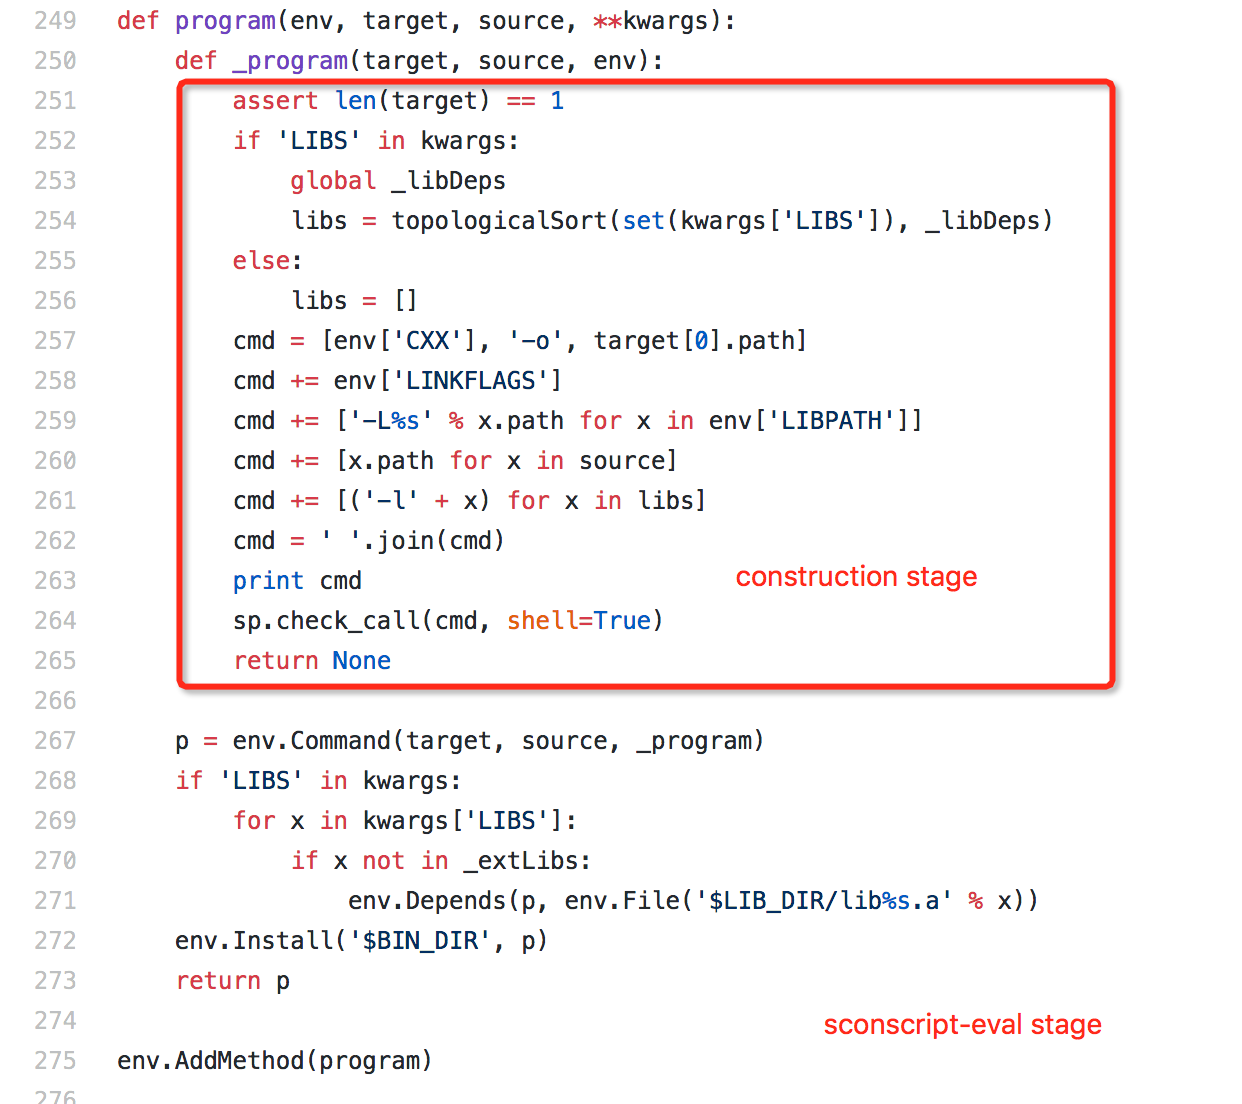
\includegraphics[width=0.95\textwidth,height=0.85\textheight]{stages.png}
  \end{center}
\end{frame}

\begin{frame}
  \frametitle{Construction stage}

  \begin{block}{Basic questions}
    \begin{itemize}
    \item What to build?
    \item What should be built?
    \end{itemize}
  \end{block}
\end{frame}

\begin{frame}[fragile]
  \frametitle{Construction stage}

  \begin{block}{What to build?}
    \begin{itemize}
    \item Specify a file: \mint{text}|scons build/debug64/bin/sqlonline_common_unittest|
    \item Specify a dir: \mint{text}|scons build/debug64/sqlonline/master/|
    \item Specify an alias: \mint{text}|scons SQLOL_ALL|
    \item Specify defaults: \mint{text}|scons|
    \end{itemize}
  \end{block}
  \note[item]{
    Specifying a dir means what to build all things under that dir.}
  \note[item]{
    Depending on a dir means that dir must be existent.}
  \note[item]{
    Specifying nothing means specifying built-in `default' alias.}
  \note[item]{
    Apsara scons allows commands like `scons fuxi', which are both unnecessary and misunderstanding.}
\end{frame}

\begin{frame}[fragile]
  \frametitle{Construction stage}

  \begin{block}{What should be built?}
    \begin{itemize}
    \item Once built, each target has a signature, including timestamp and MD5.
    \item .sconsign.dblite: all built targets, with their signatures and dependencies and builders
    \item If \mintinline{python}|CacheDir| specified, a cached target will be applied.
      \begin{txt*}{gobble=8}
        $ find scons-cache
        scons-cache/F6
        scons-cache/F6/f6af98b6859101b4724b6f96e500d442
        scons-cache/F6/f6f60ebbcaf7b8e08dfcb47d5ef70075
        scons-cache/5B
        scons-cache/5B/5bdc8181f37191d2b47bac6f28a55494
        scons-cache/5B/5bad97e866c4f3f9f50a4ead679859a9
      \end{txt*}
      %$
    \end{itemize}
  \end{block}
  \note[item]{
    For a target, if all its upstreams and the builder are not changed, it will not be rebuilt.}
  \note[item]{
    Signature contents are decided by `\mintinline{python}|env.Decider('MD5-timestamp')|'.}
  \note[item]{
    SCons cache works for all targets, while ccache works not for gcc-generated objects.}
\end{frame}

\begin{frame}[fragile]
  \frametitle{SConscript-eval stage}

  \begin{block}{files, dirs}
    \begin{itemize}
    \item \mintinline{python}|env.File('$BIN_DIR/apsara_log_conf.json')|%$
    \item \mintinline{python}|env.Glob('*.cpp')|
    \item \mintinline{python}|env.Dir('#')|
    \item For file/dir nodes, we are usually interested in their \mintinline{python}{.path} and \mintinline{python}{.abspath} members.
    \end{itemize}
  \end{block}
  \note[item]{
    env.File() and env.Dir() will substitude `\#' for the project root,
    and `\mintinline{text}|$XYZ|' for value of env['XYZ'].} %$
\end{frame}

\begin{frame}[fragile]
  \frametitle{SConscript-eval stage}

  \begin{block}{alias}
    \begin{itemize}
    \item named aliases: \mintinline{python}|env.Alias('SQLOL_ALL', log_cfg)|
    \item default alias:
      \begin{itemize}
      \item \mintinline{python}|Default(None)|:  default nothing
      \item \mintinline{python}|Default(xyz)|: add xyz to default
      \end{itemize}
    \end{itemize}
  \end{block}
\end{frame}

\begin{frame}[fragile]
  \frametitle{SConscript-eval stage}

  \begin{block}{Requires, Depends}
    \begin{itemize}
    \item \mintinline{python}|Depends(a, x)|:
      the construction on `\mintinline{python}|a|' depends on the content of `\mintinline{python}|x|'.
    \item \mintinline{python}|Requires(a, x)|:
      the construction on `\mintinline{python}|a|' requires the existence of `\mintinline{python}|x|'.
    \item<2-> \mintinline{python}|Depends([a,b], x)| =? \mintinline{python}|Depends(a, x); Depends(b, y)|
    \item<3-> \mintinline{python}|Depends(a, [x,y])| =? \mintinline{python}|Depends(a, x); Depends(b, y)|
    \end{itemize}
  \end{block}
  \note[item]<3>{
    In \mintinline{python}|Depends(a, [x,y])|,
    when the order of `\mintinline{python}|[x,y]|' changes, `\mintinline{python}|a|' must be rebuilt.}
\end{frame}

\begin{frame}[fragile]
  \frametitle{SConscript-eval stage}

  \begin{block}{external-command builder}
    \begin{py*}{gobble=6}
      bld = Builder(action = 'foobuild < $SOURCE > $TARGET')
      env.Append(BUILDERS = {'Foo' : bld})
      env.Foo('foo.out', 'foo.in')
    \end{py*}
  \end{block}
\end{frame}

\begin{frame}[fragile]
  \frametitle{SConscript-eval stage}

  \begin{block}{python builder}
    \begin{py*}{gobble=6}
      def foobuild(target, source, env):
        # Code to build "target" from "source"
        return None
      bld = Builder(action = foobuild)
      env = Environment(BUILDERS = {'Foo' : bld})
      env.Foo('foo.out', 'foo.in')
    \end{py*}
  \end{block}
  \note[item]{
    Because of GIL, python builder is of less parallelling.}
\end{frame}

\begin{frame}[fragile]
  \frametitle{SConscript-eval stage}

  \begin{block}{unamed builder}
    \begin{py*}{gobble=6}
      env.Command('foo.out', 'foo.in', "foobuid < $SOURCE > $TARGET")

      def foobuild(target, source, env):
        # Whatever it takes to build
        return None
      env.Command('foo.out', 'foo.in', foobuild)
    \end{py*}
  \end{block}
\end{frame}

\subsection{Diagnose}

\begin{frame}[fragile]
  \frametitle{Diagnose}

  \begin{block}{performance tuning}
    \begin{txt*}{gobble=6}
      $ scons mode=release --debug=time
      SConscript:/home/admin/workspace/ots/build/release64/ots/protocol/SConscript  took 21.659 ms
      ...
      SConscript:/home/admin/workspace/ots/build/release64/SConscript  took 15477.719 ms
      SConscript:/home/admin/workspace/ots/SConstruct  took 36770.681 ms
      scons: done reading SConscript files.
      scons: Building targets ...
      ...
      Command execution time: build/release64/sqlonline/master/sqlonline_master: 73.548500 seconds
      ...
      scons: done building targets.
      Total build time: 940.854440 seconds
      Total SConscript file execution time: 39.401208 seconds
      Total SCons execution time: 3.983987 seconds
      Total command execution time: 897.469245 seconds
    \end{txt*}
    %$
  \end{block}
\end{frame}

\begin{frame}[fragile]
  \frametitle{Diagnose}

  \begin{block}{why something is rebuilt?}
    \begin{txt*}{gobble=6}
      $ scons mode=release --debug=explain
      ...
      scons: rebuilding `build/release64/sqlonline/common/libsqlonline_common_t_static.a' because:
           `build/release64/sqlonline/common/common.os' changed
           `build/release64/sqlonline/common/sqlonline_compressor.os' changed
           `build/release64/sqlonline/common/profile/hardware_usage.os' changed
      ...
    \end{txt*}
    %$
  \end{block}
\end{frame}

\begin{frame}[fragile]
  \frametitle{Diagnose}

  \begin{block}{why something is rebuilt?}
    \begin{txt*}{gobble=6}
      $ scons mode=release --tree=prune
      ...
      +-build/release64/ots/protocol/ots_protocol.4.pb.h
        +-build/release64/ots/protocol/ots_protocol.4.proto
        +-dist/apsara/bin/protoc
      ...
    \end{txt*}
    %$
  \end{block}
\end{frame}

\subsection{Dark Side of SCons}

\begin{frame}[fragile]
  \frametitle{Python is a two-side blade}

  \begin{block}{Extremely flexible}
    \begin{py*}{gobble=6}
      def UpdateMethod(env, methodName, func):
        env.RemoveMethod(getattr(env, methodName))
        env.AddMethod(func, methodName)

      def WrapMethod(wrapped, self, *args, **kwargs):
        localTarget = wrapped(self, *args, **kwargs)
        self.Alias('SQLOL_ALL', localTarget)

      UpdateMethod(tenv, 'tProgram',
        partial(WrapMethod, tenv.tProgram.method))
    \end{py*}
    
    But it is too flexible to integrate with IDEs.
  \end{block}
  \note[item]{
    Every target produced by tProgram is added to SQLOL\_ALL alias.}
  \note[item]{
    Ant/Maven is good at IDE integration, but many things they can't do.}
\end{frame}

\begin{frame}[fragile]
  \frametitle{Portability}

  \begin{block}{~}
    \begin{itemize}
    \item SCons core, because of its pythonic purity, is portable.
    \item SConscripts, their portability depend on their authors.
      \begin{py*}{gobble=8}
        compiler, version = detect_compiler()
        if compiler == 'g++':
          flags['CXXFLAGS'].append('--std=gnu++03')
          if version >= [4, 9, 0]:
            flags['CCFLAGS'].extend(['-fsanitize=address', '-fvar-tracking-assignments'])
            flags['LINKFLAGS'].extend(['-fsanitize=address'])
        else:
          print compiler, version
          assert False, 'unsupport compiler'
      \end{py*}
    \end{itemize}
  \end{block}
\end{frame}

\begin{frame}
  \frametitle{Safe build}

  \begin{block}{~}
    \begin{itemize}
    \item VariantDir() automatically hardlinks files to the build directory.
    \item Glob() selects files both in the source directory and in the build directory.
    \item<2-> Here is the problem: Glob('*.cpp') will select a file which is deleted in the source directory.
    \item<2-> My solution:
      \begin{itemize}
      \item Not to use VariantDir().
      \item Softlinks all files in the soure directory to the build directory.
      \item From the beginning of a build, clean all softlinks in the build directory.
      \end{itemize}
    \end{itemize}
  \end{block}
\end{frame}

\begin{frame}
  \frametitle{Safe build}

  \begin{block}{~}
    \begin{itemize}
    \item But aPackage() is still bleeding.
      \begin{itemize}
      \item It is hard to distinguish a file which is necessary to this build from a file just-be-there.
      \item The final solution: forbid incremental building.
        \begin{itemize}
        \item with the help of caching
        \end{itemize}
      \end{itemize}
    \end{itemize}
  \end{block}
\end{frame}

\section{Conclusions}

\begin{frame}
  \frametitle{Flavours of build tools}

  \begin{block}{Scripting}
    \begin{itemize}
    \item Origin from Makefile
      \begin{itemize}
      \item Good extensibility/Poor IDE integration
      \item Lack of scalable dependency graph
      \item Deeply depends on the environment
      \end{itemize}
    \item Upstreams to Makefile
      \begin{itemize}
      \item automake: more portability
      \item cmake/bazel: DSL to draw dependency graph
      \end{itemize}
    \item Downstreams to Makefile
      \begin{itemize}
      \item distcc: parallelling
      \item ccache: caching
      \end{itemize}
    \end{itemize}
  \end{block}
  \note[item]{
    Makefile has just one stage.
    It employs parallel structures.
    To amend the missing stage, cmake decides to generate Makefile.}
\end{frame}

\begin{frame}
  \frametitle{Flavours of build tools}

  \begin{block}{Configurations}
    \begin{itemize}
    \item Origin from Ant
      \begin{itemize}
      \item Good IDE integration
      \item Usually hard for human readers
      \item Lack of scalable dependency graph
      \end{itemize}
    \item Maven automatically downloads plugins and 3rd-party libraries.
      \begin{itemize}
        \item jar hell
      \end{itemize}
    \end{itemize}
  \end{block}
\end{frame}

\begin{frame}
  \frametitle{Flavours of build tools}

  \begin{block}{General-purpose language}
    \begin{itemize}
    \item Origin from SCons
      \begin{itemize}
      \item Leverage a general-purpose programming language
      \item Focus on scalable dependency graph
      \end{itemize}
    \item Graddle,
      \begin{itemize}
      \item introduces philosophy of SCons to Java world.
      \item Leverages ecosystem of Maven.
      \end{itemize}
    \end{itemize}
  \end{block}
\end{frame}

\begin{frame}
  \frametitle{}
  \begin{center}
    \Huge
    Questions?
  \end{center}
\end{frame}

\end{document}

